 \begin{savequote}[8cm]
\textlatin{Cor animalium, fundamentum e\longs t vitæ, princeps omnium, Microco\longs mi Sol, a quo omnis vegetatio dependet, vigor omnis \& robur emanat.}

The heart of animals is the foundation of their life, the sovereign of everything within them, the sun of their microcosm, that upon which all growth depends, from which all power proceeds.
  \qauthor{--- William Harvey \cite{harvey_exercitatio_1628}}
\end{savequote}

\chapter{\label{app:perf}performance}

\minitoc

\section{TKI comparisons for the SFGD-$\mu$ sub-sample for the $\numucczpiop$ selection}
\label{sec:app-tki-sfgd-mu}

     \begin{figure}
     \centering
          \begin{subfigure}[b]{\dbfigwid\textwidth}
               \centering
               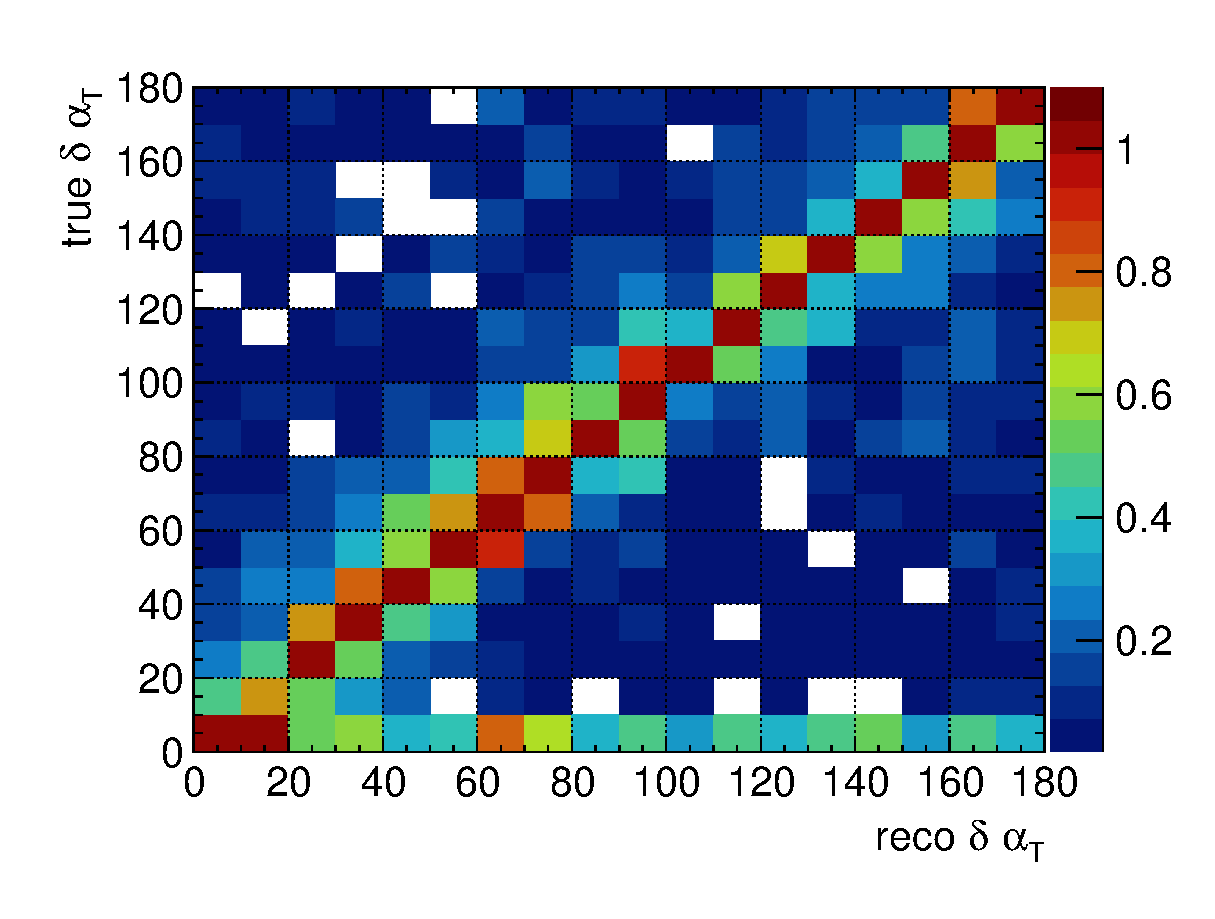
\includegraphics[width=\textwidth]{figures/perf/tki/dalphat_colnor_resmat_al10_sfgmu.eps}
               \caption{$\dat$ before ESC}
               \label{subfig:esc-dalpha-bfesc-sfgmu}
          \end{subfigure}         
          \begin{subfigure}[b]{\dbfigwid\textwidth}
               \centering
               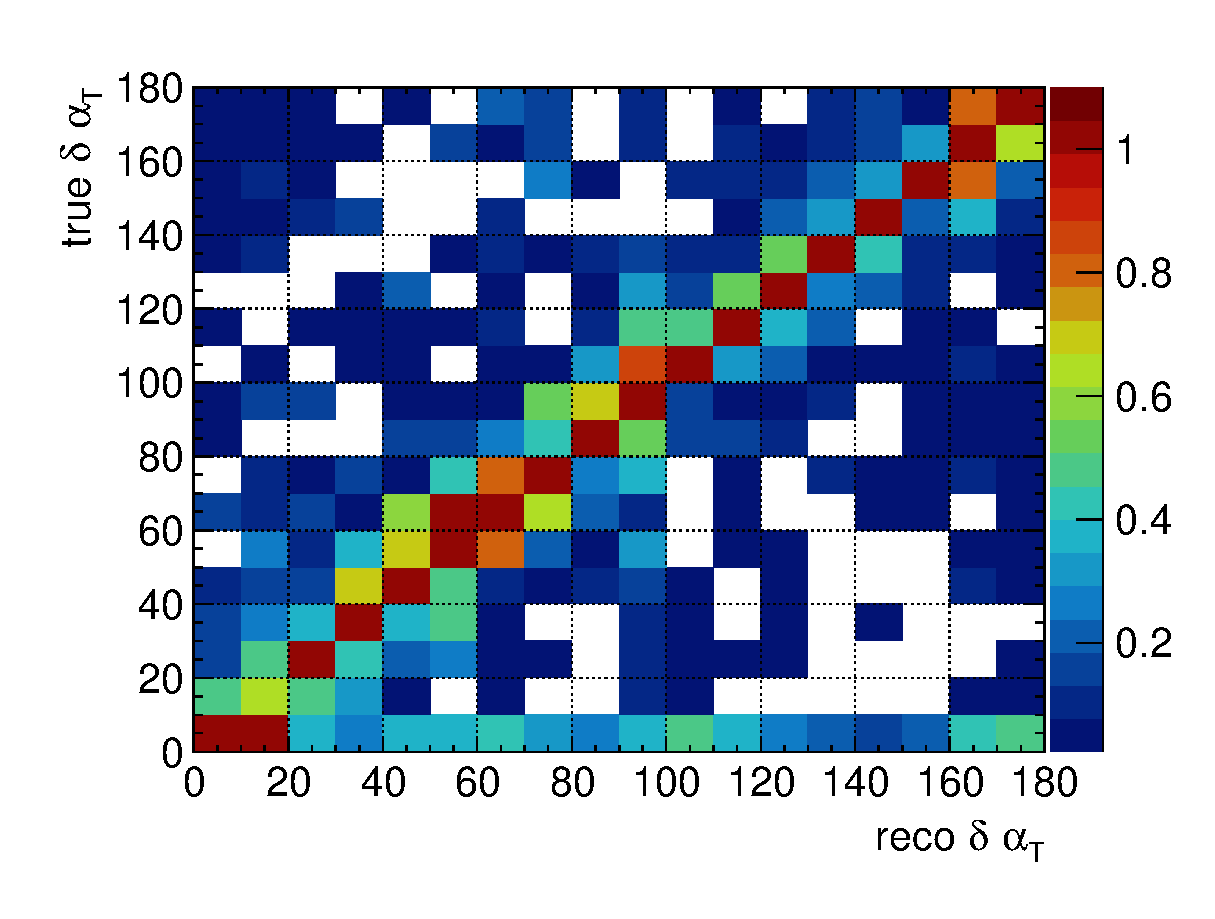
\includegraphics[width=\textwidth]{figures/perf/tki/dalphat_colnor_resmat_al11_sfgmu.eps}
               \caption{$\dat$ after ESC}
               \label{subfig:esc-dalpha-afesc-sfgmu}
          \end{subfigure}
          \\
          \begin{subfigure}[b]{\dbfigwid\textwidth}
               \centering
               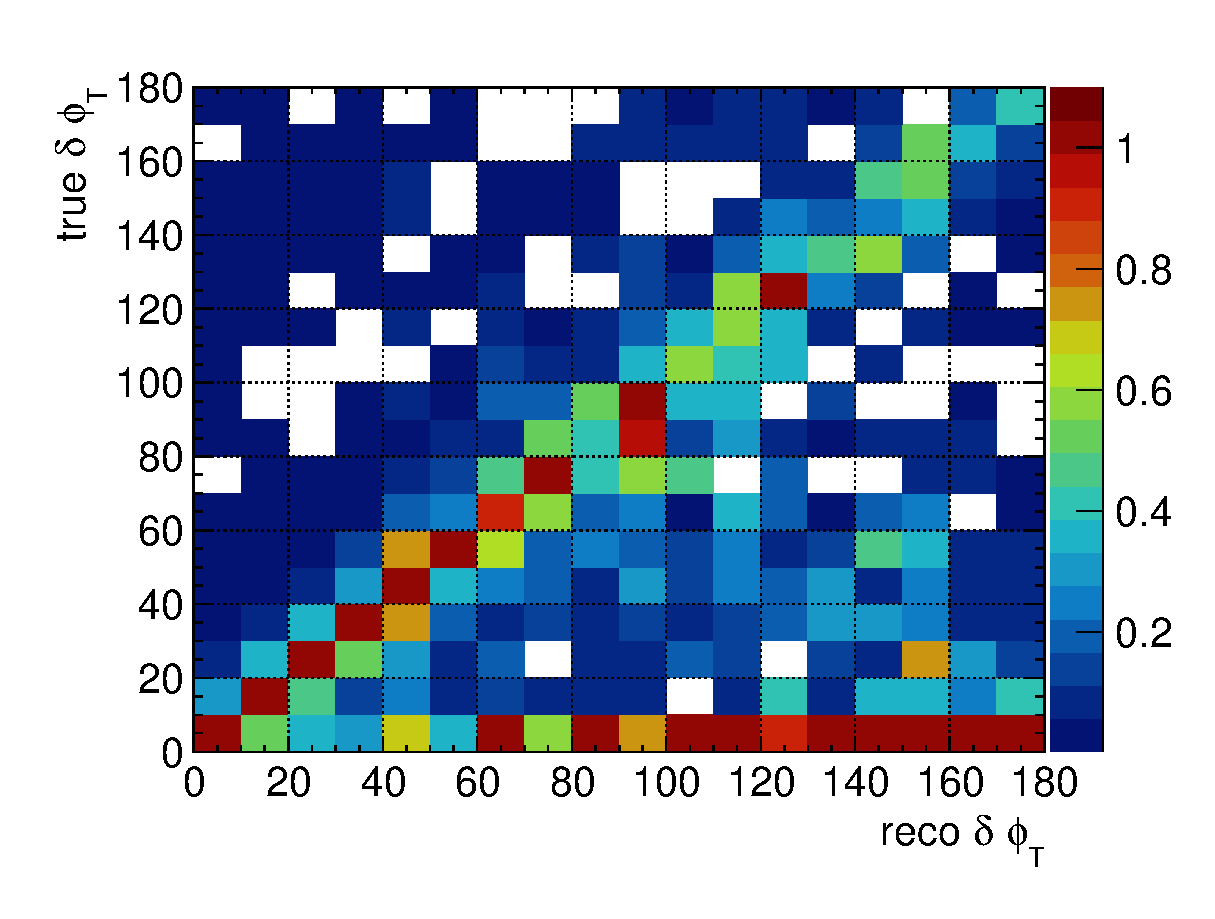
\includegraphics[width=\textwidth]{figures/perf/tki/dphitcolnor_resmat_al10_sfgmu.eps}
               \caption{$\dphit$ before ESC}
               \label{subfig:esc-dphit-bfesc-sfgmu}
          \end{subfigure}
          \begin{subfigure}[b]{\dbfigwid\textwidth}
               \centering
               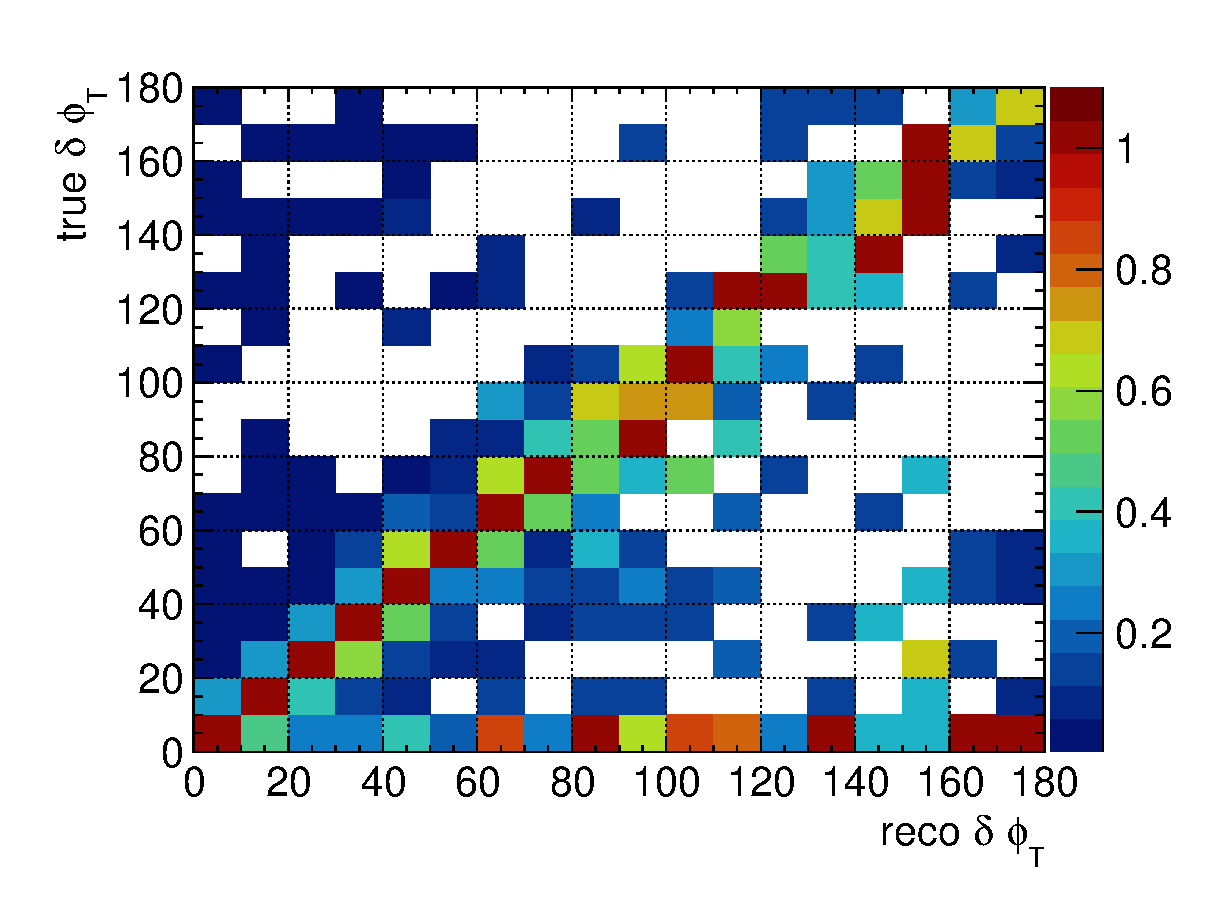
\includegraphics[width=\textwidth]{figures/perf/tki/dphitcolnor_resmat_al11_sfgmu.eps}
               \caption{$\dphit$ after ESC}
               \label{subfig:esc-dphit-afesc-sfgmu}
          \end{subfigure}
          \\
          \begin{subfigure}[b]{\dbfigwid\textwidth}
               \centering
               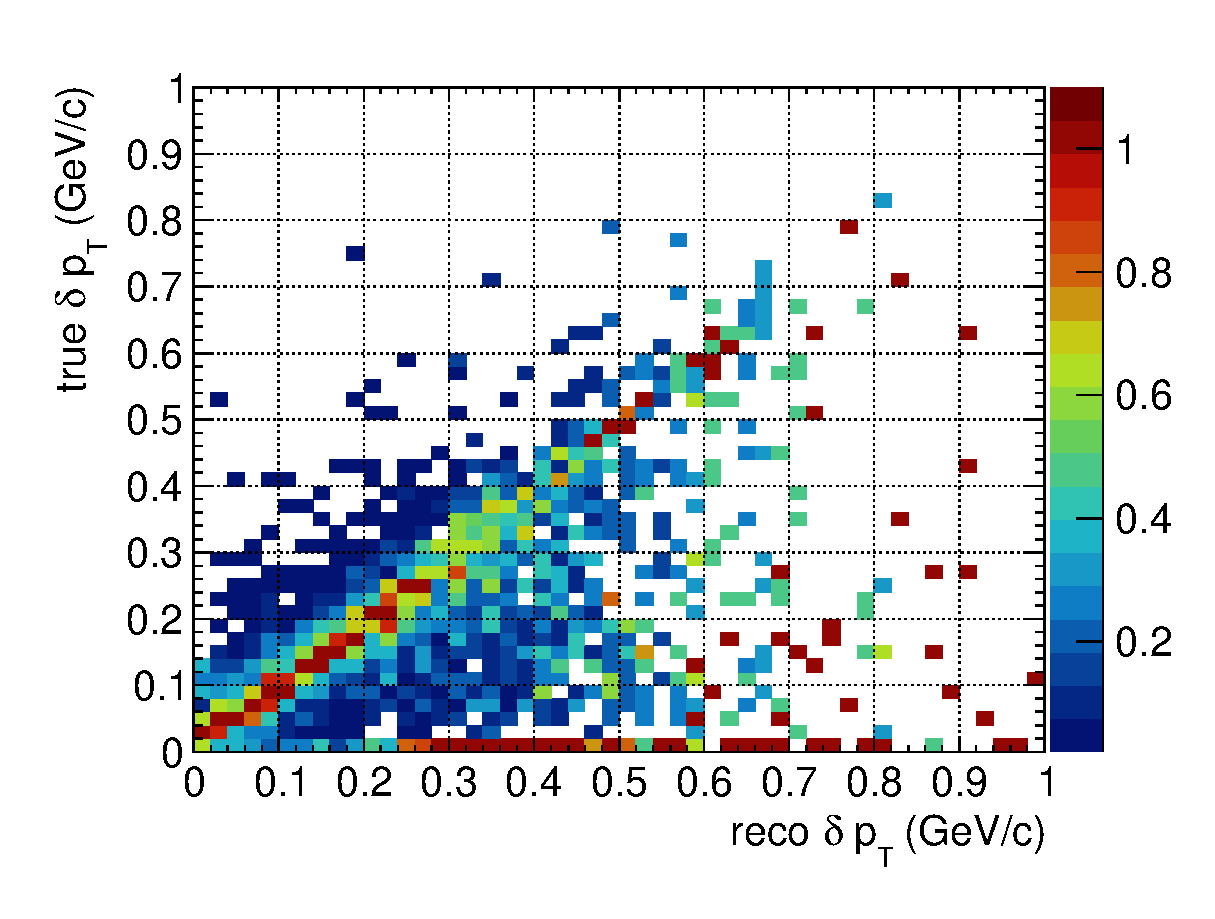
\includegraphics[width=\textwidth]{figures/perf/tki/dpt_colnor_resmat_al10_sfgmu.eps}
               \caption{$\dpt$ before ESC}
               \label{subfig:esc-dpt-bfesc-sfgmu}
          \end{subfigure}
          \begin{subfigure}[b]{\dbfigwid\textwidth}
               \centering
               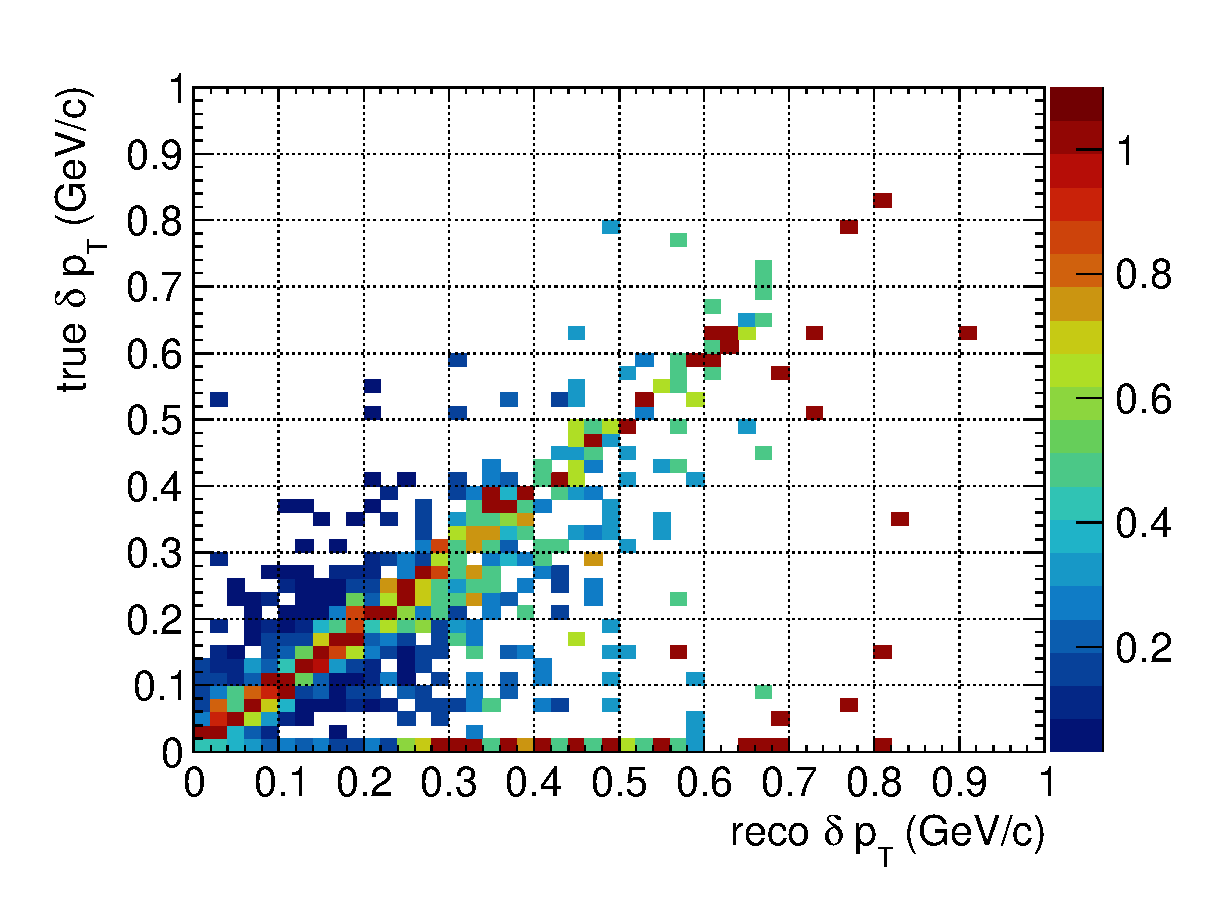
\includegraphics[width=\textwidth]{figures/perf/tki/dpt_colnor_resmat_al11_sfgmu.eps}
               \caption{$\dpt$ after ESC}
               \label{subfig:esc-dpt-afesc-sfgmu}
          \end{subfigure}
          \\
          \begin{subfigure}[b]{\dbfigwid\textwidth}
               \centering
               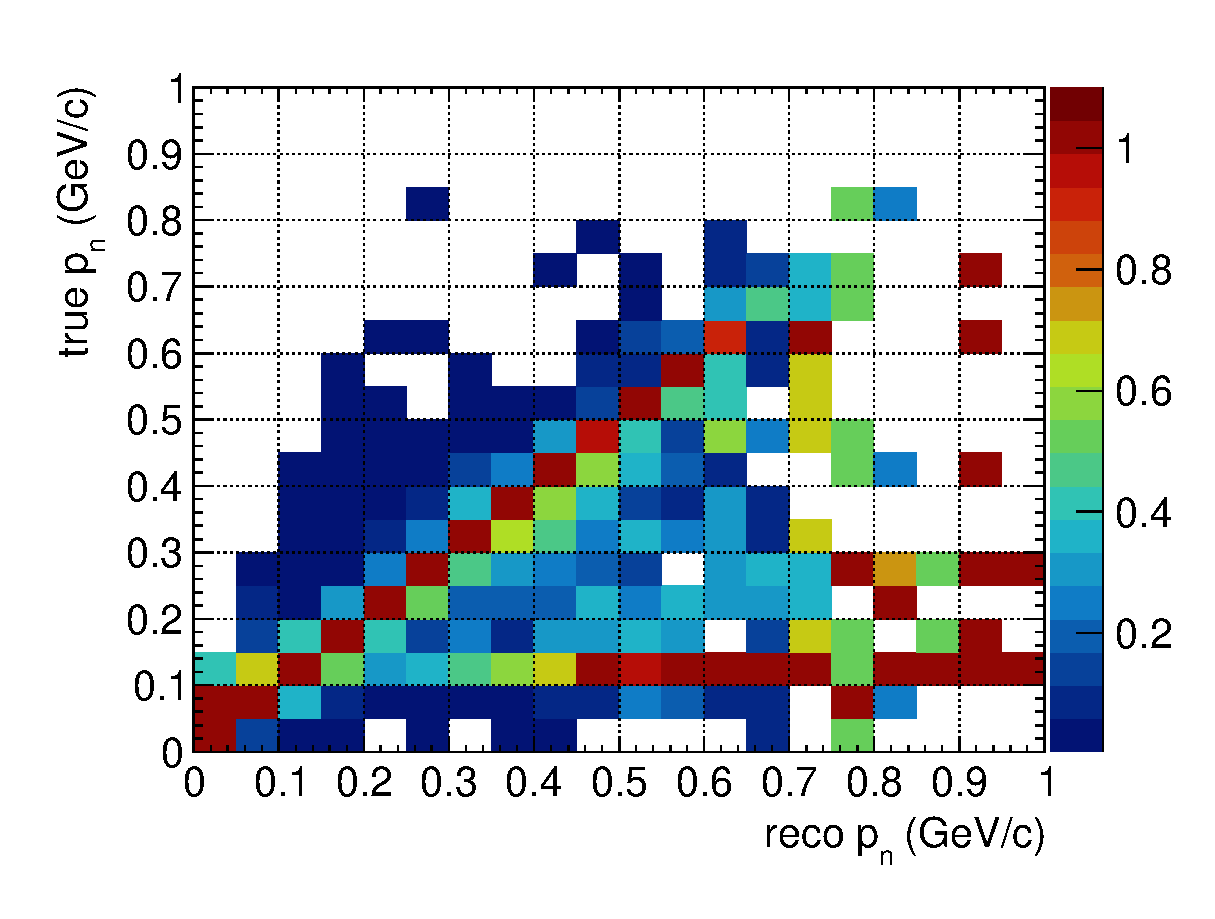
\includegraphics[width=\textwidth]{figures/perf/tki/pn_colnor_resmat_al10_sfgmu.eps}
               \caption{$\pn$ before ESC}
               \label{subfig:esc-pn-bfesc-sfgmu}
          \end{subfigure}
          \begin{subfigure}[b]{\dbfigwid\textwidth}
               \centering
               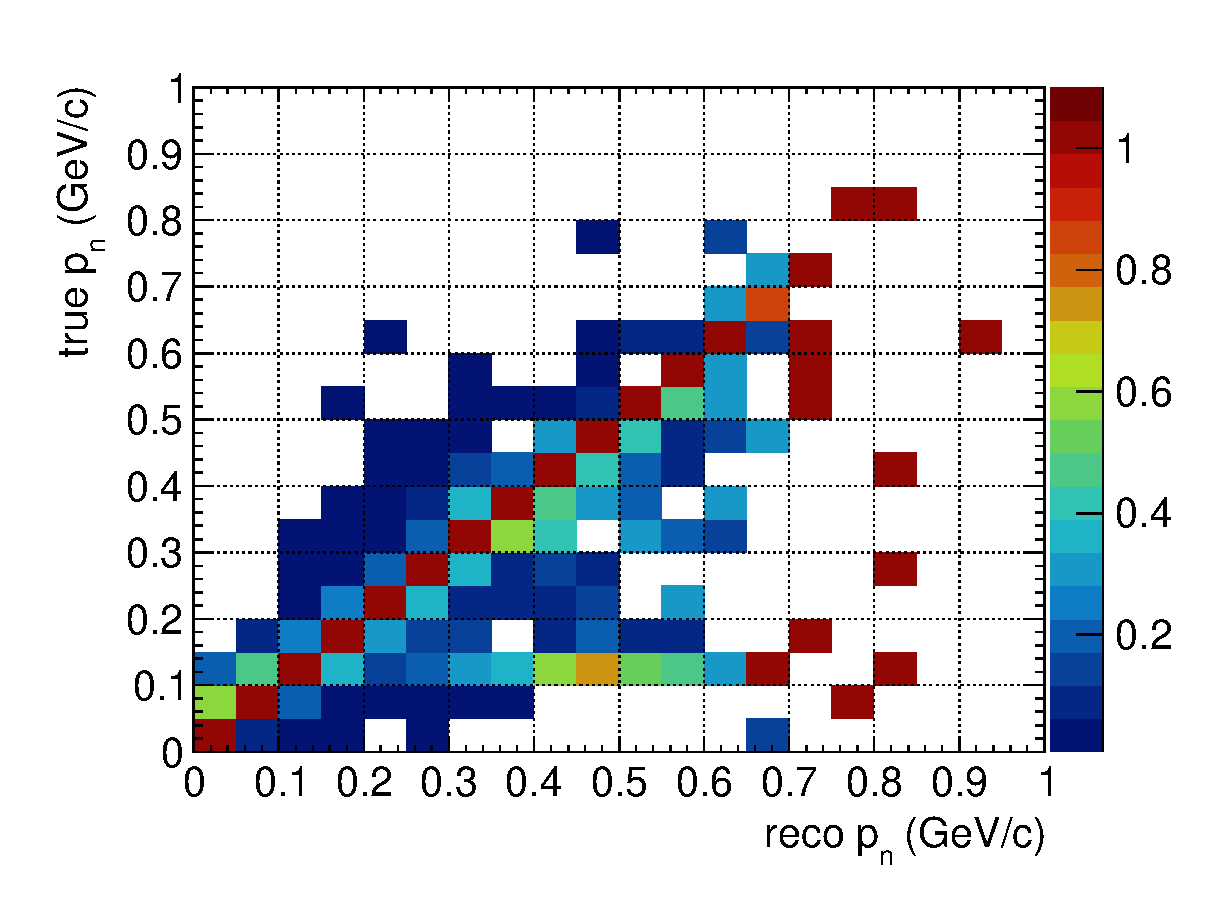
\includegraphics[width=\textwidth]{figures/perf/tki/pn_colnor_resmat_al11_sfgmu.eps}
               \caption{$\pn$ after ESC}
               \label{subfig:esc-pn-afesc-sfgmu}
          \end{subfigure}
          \caption{TKI variables before and after ESC for the $\numucczpiop$ selection for the SFGD-$\mu$ sub-sample.}
          \label{fig:mc-tki-0pi-esc-sfgmu}
     \end{figure}


     \begin{figure}
          \begin{subfigure}[b]{\dbfigwid\textwidth}
               \centering
               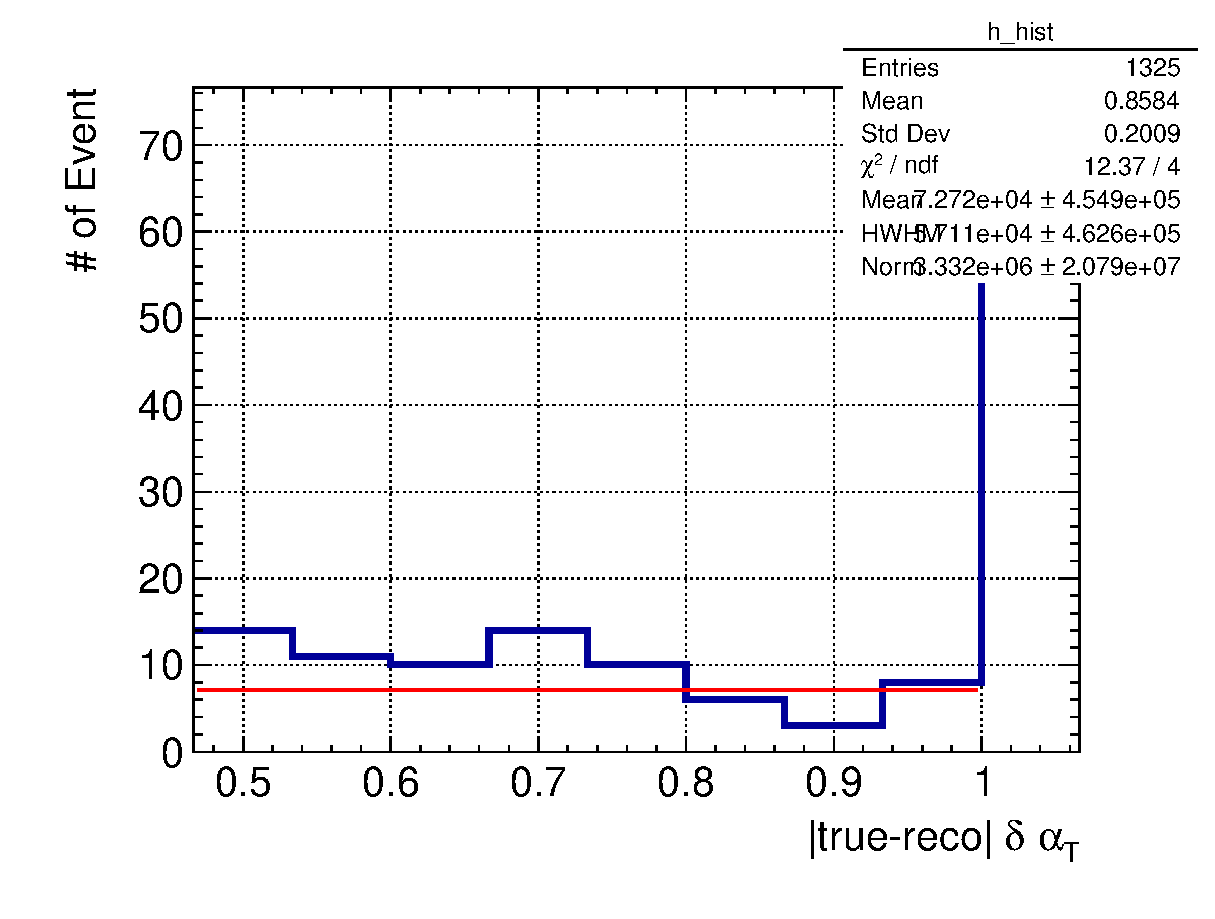
\includegraphics[width=\textwidth]{figures/perf/tki/dalphat_rat_hist_al11_sfgmu.eps}
               \caption{$\dat$ before muon bias correction}
               \label{subfig:esc-dalpha-bfmu-sfgmu}
          \end{subfigure}         
          \begin{subfigure}[b]{\dbfigwid\textwidth}
               \centering
               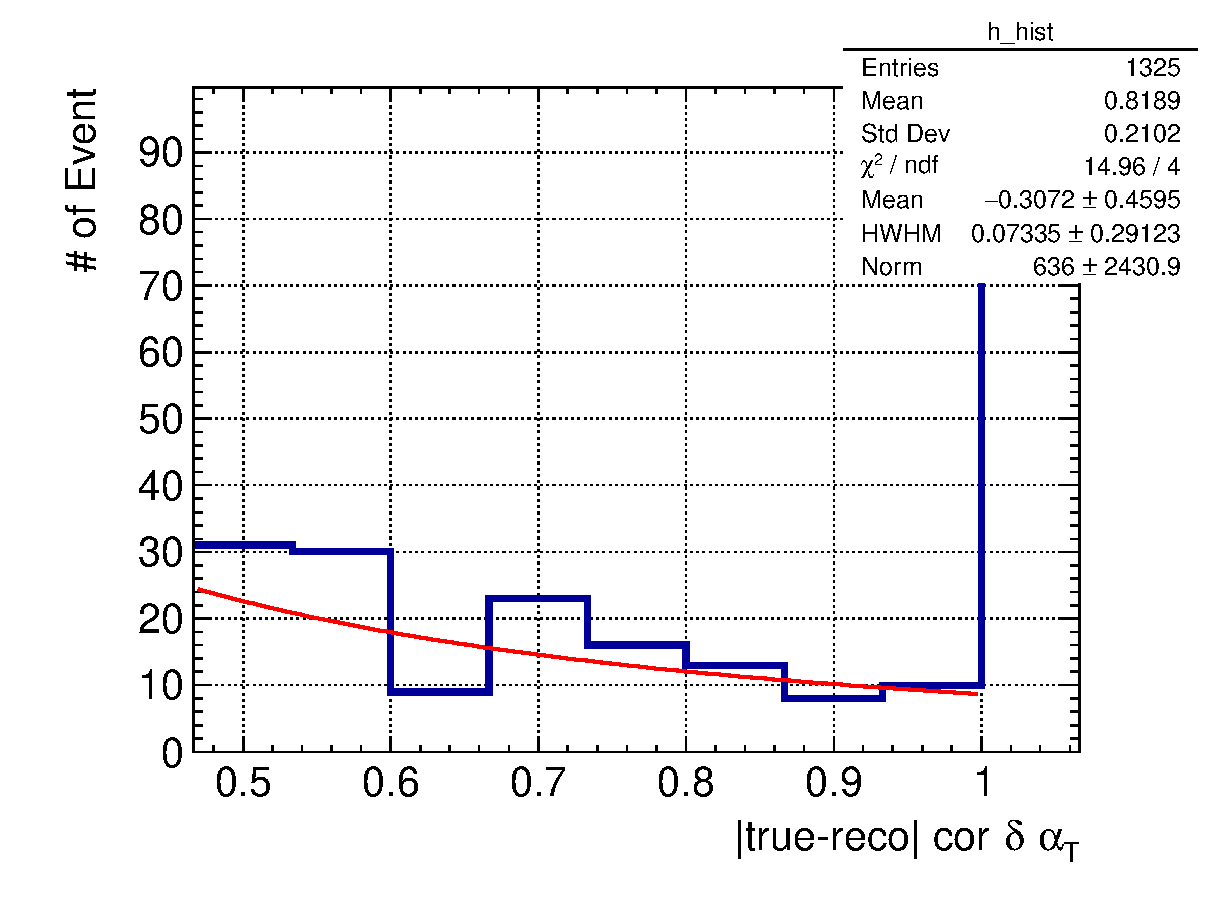
\includegraphics[width=\textwidth]{figures/perf/tki/cor_dalphat_rat_hist_al11_sfgmu.eps}
               \caption{$\dat$ after muon bias correction}
               \label{subfig:esc-dalpha-afmu-sfgmu}
          \end{subfigure}
          \\
          \begin{subfigure}[b]{\dbfigwid\textwidth}
               \centering
               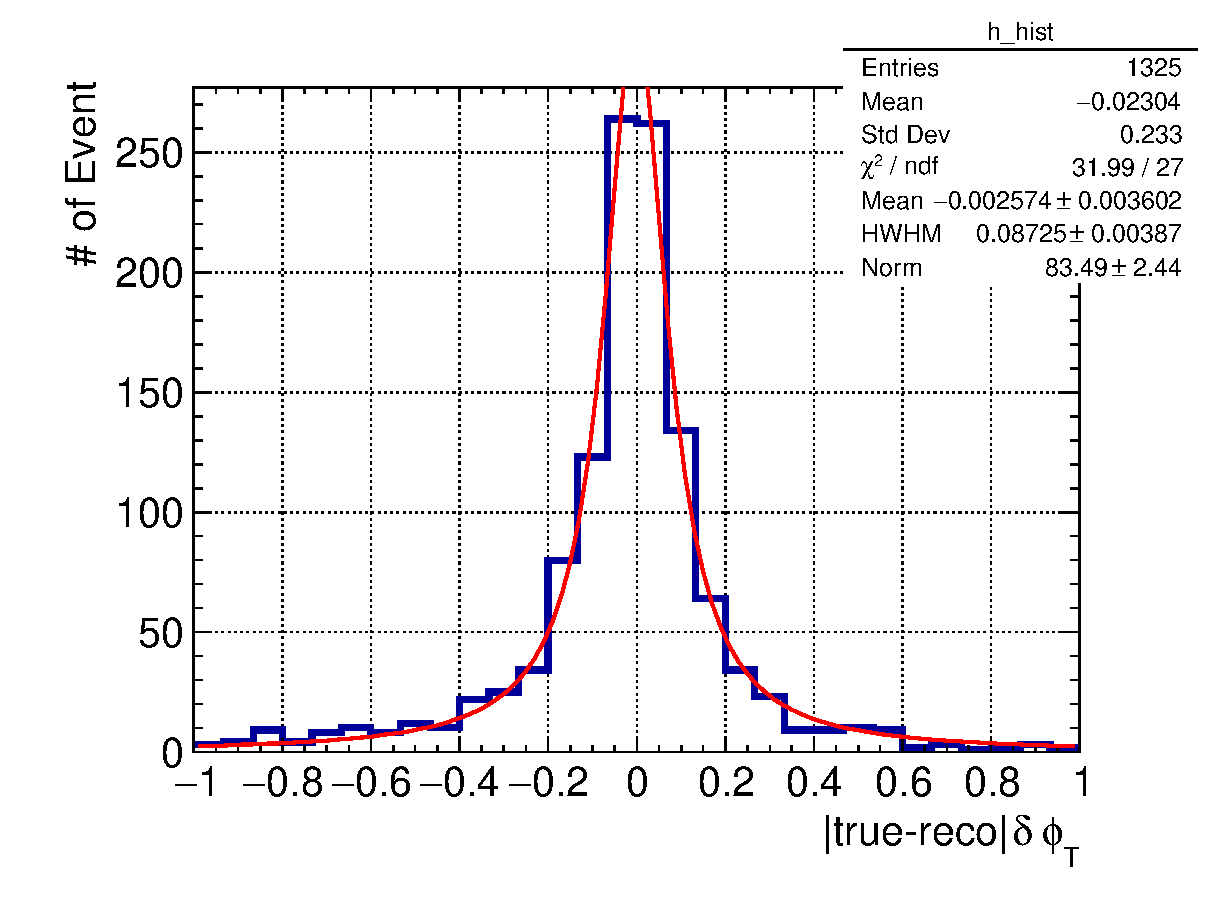
\includegraphics[width=\textwidth]{figures/perf/tki/dphit_rat_hist_al11_sfgmu.eps}
               \caption{$\dphit$ before muon bias correction}
               \label{subfig:esc-dphit-bfmu-sfgmu}
          \end{subfigure}
          \begin{subfigure}[b]{\dbfigwid\textwidth}
               \centering
               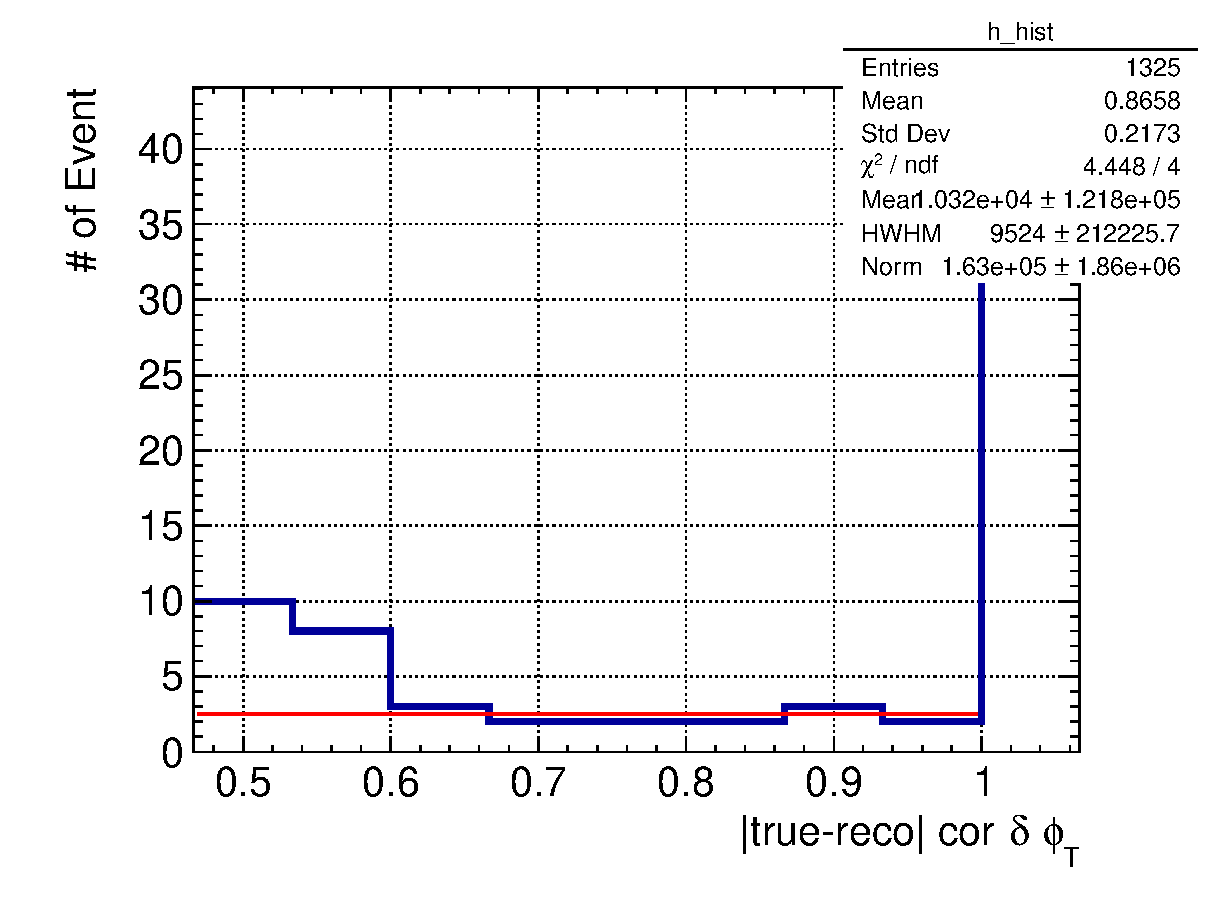
\includegraphics[width=\textwidth]{figures/perf/tki/cor_dphit_rat_hist_al11_sfgmu.eps}
               \caption{$\dphit$ after muon bias correction}
               \label{subfig:esc-dphit-afmu-sfgmu}
          \end{subfigure}
          \\
          \begin{subfigure}[b]{\dbfigwid\textwidth}
               \centering
               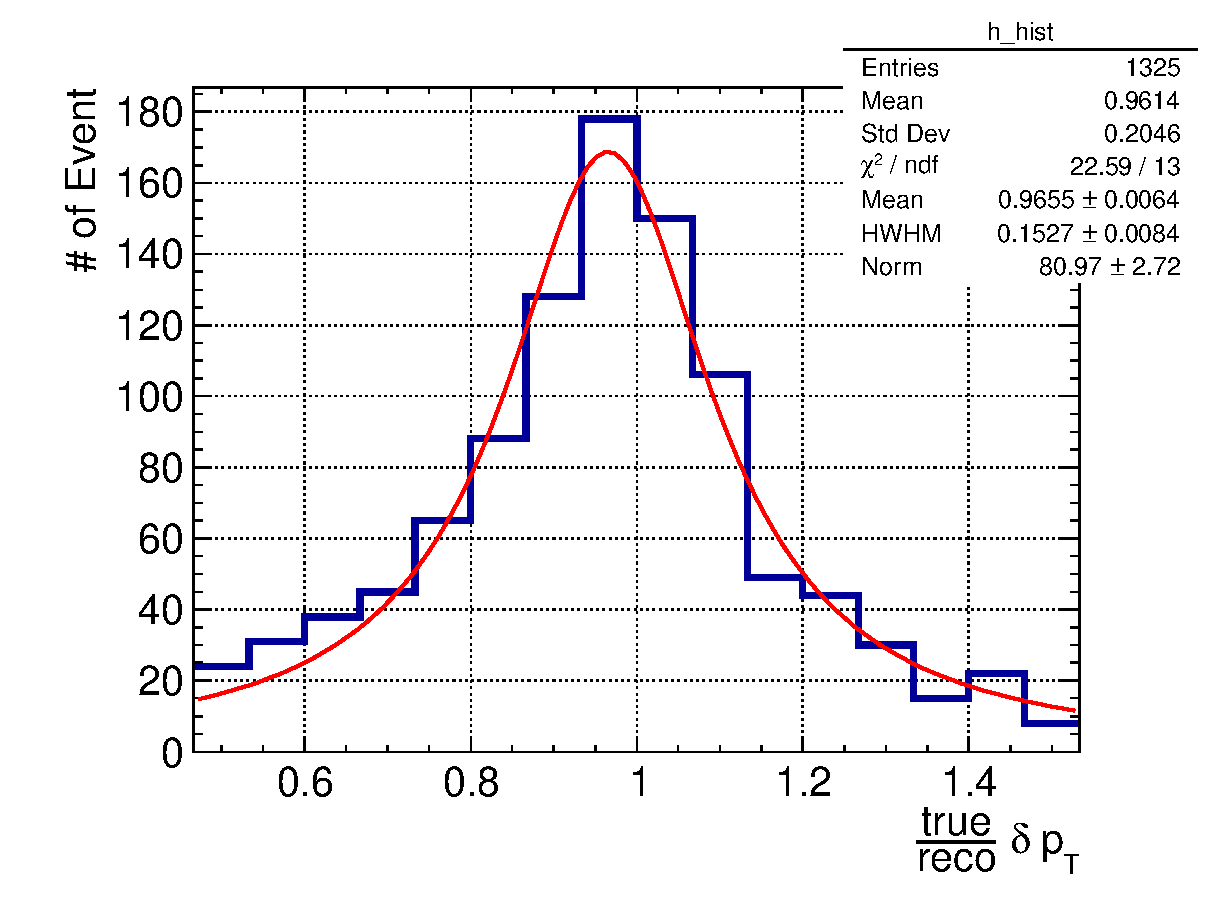
\includegraphics[width=\textwidth]{figures/perf/tki/dpt_rat_hist_al11_sfgmu.eps}
               \caption{$\dpt$ before muon bias correction}
               \label{subfig:esc-dpt-bfmu-sfgmu}
          \end{subfigure}
          \begin{subfigure}[b]{\dbfigwid\textwidth}
               \centering
               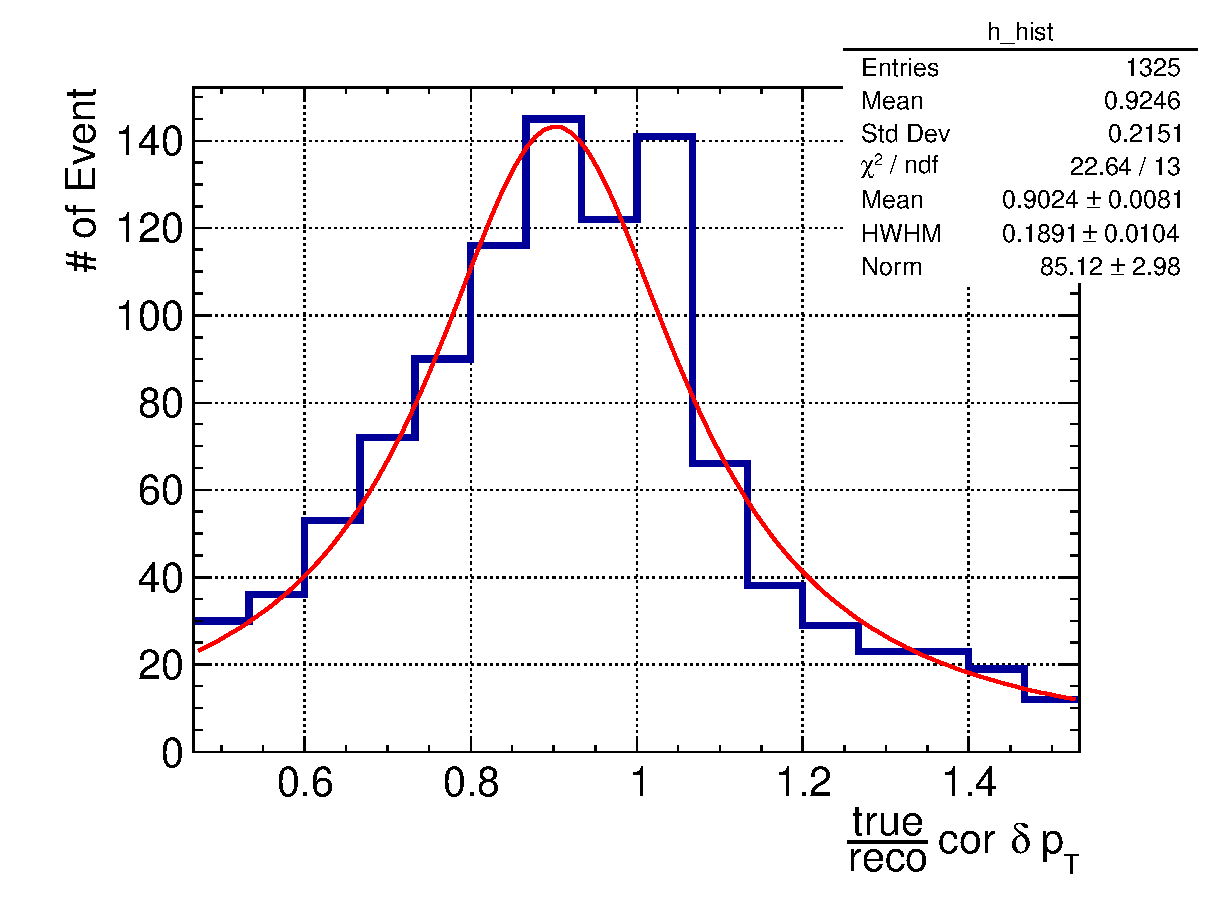
\includegraphics[width=\textwidth]{figures/perf/tki/cor_dpt_rat_hist_al11_sfgmu.eps}
               \caption{$\dpt$ after muon bias correction}
               \label{subfig:esc-dpt-afmu-sfgmu}
          \end{subfigure}
          \\
          \begin{subfigure}[b]{\dbfigwid\textwidth}
               \centering
               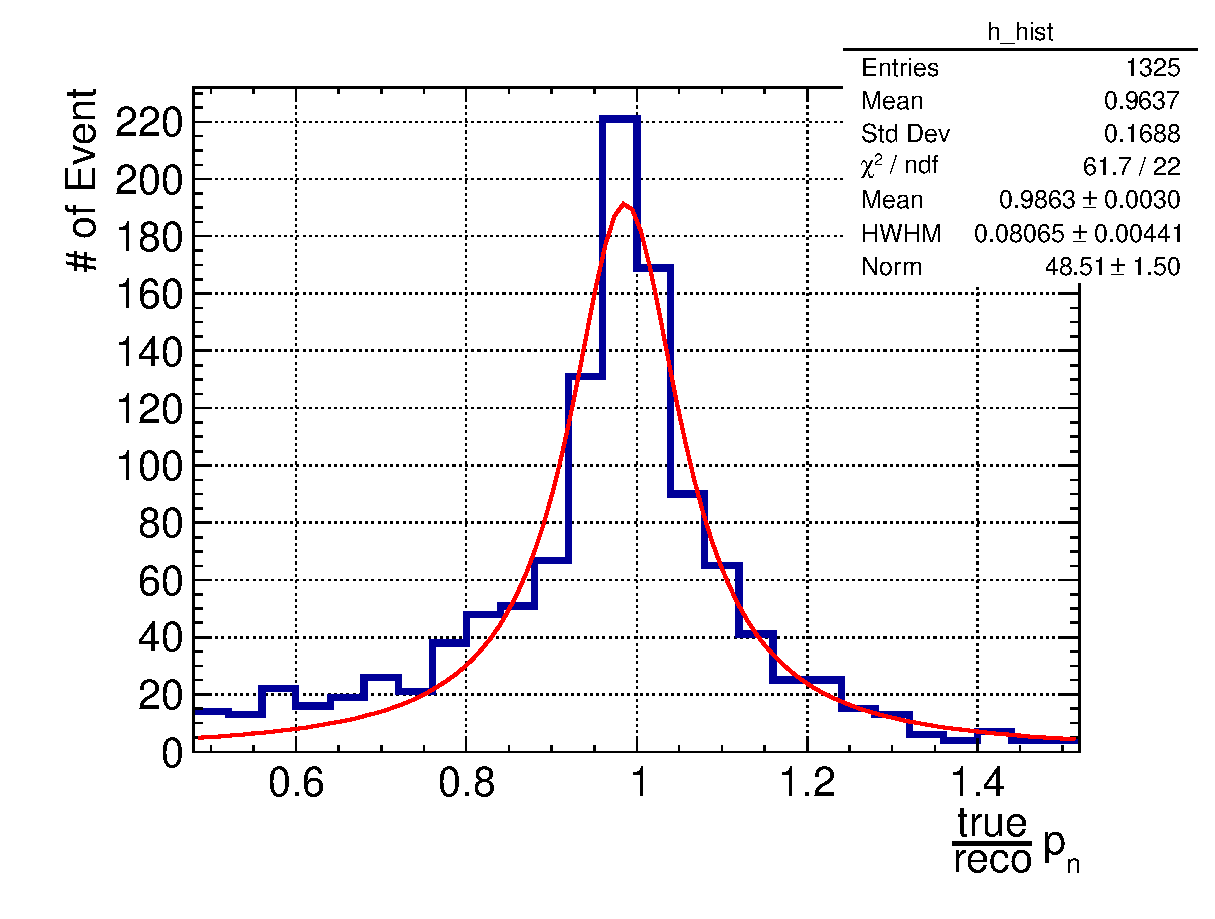
\includegraphics[width=\textwidth]{figures/perf/tki/pn_rat_hist_al11_sfgmu.eps}
               \caption{$\pn$ before muon bias correction}
               \label{subfig:esc-pn-bfmu-sfgmu}
          \end{subfigure}
          \begin{subfigure}[b]{\dbfigwid\textwidth}
               \centering
               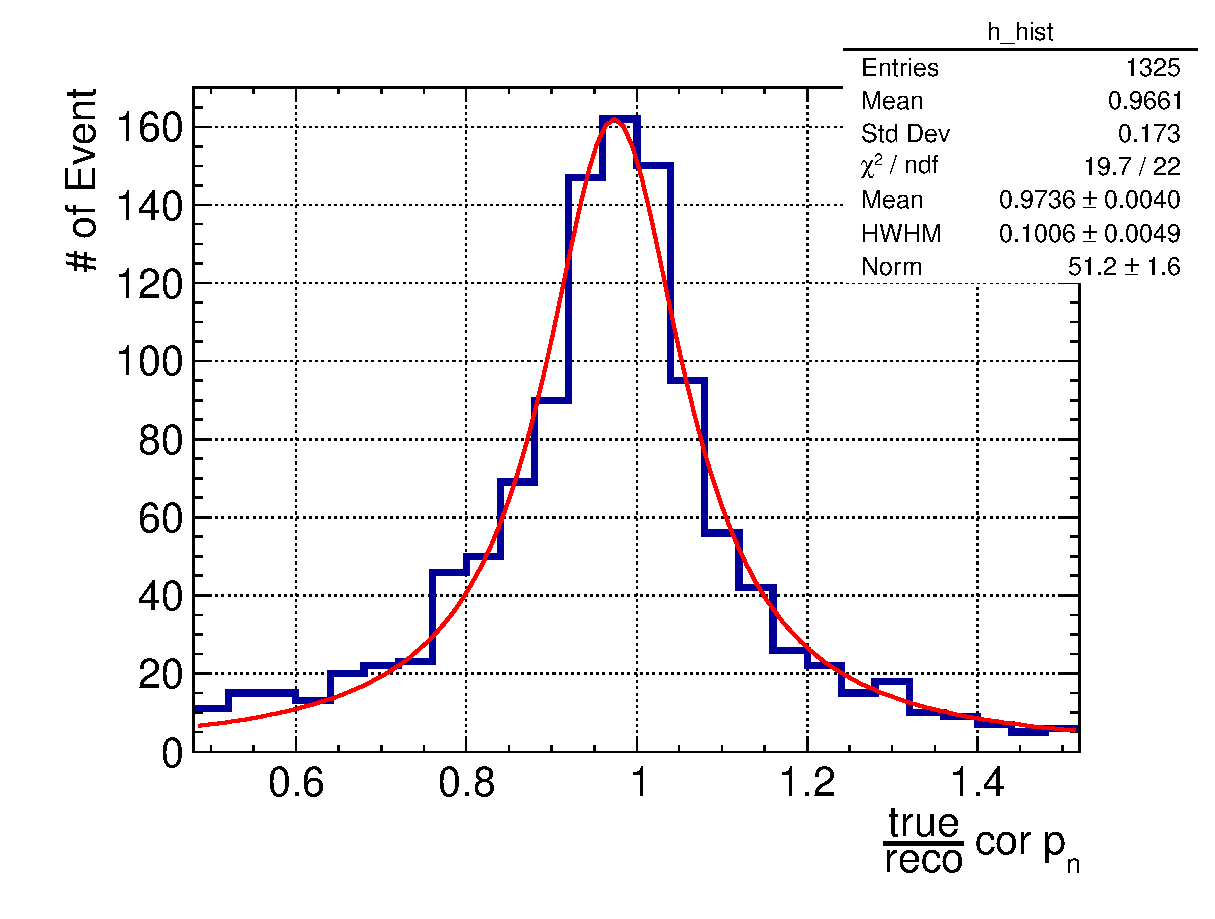
\includegraphics[width=\textwidth]{figures/perf/tki/cor_pn_rat_hist_al11_sfgmu.eps}
               \caption{$\pn$ after muon bias correction}
               \label{subfig:esc-pn-afmu-sfgmu}
          \end{subfigure}
          \caption{TKI variables before and after muon bias correction for the $\numucczpiop$ selection for the SFGD-$\mu$ sub-sample.}
          \label{fig:mc-tki-0pi-mu-sfgmu}
     \end{figure}
 